\documentclass[12pt]{article}
\newif\ifanswer\answertrue%\answerfalse% comment out to show/hide answers
\usepackage{../preamble3}% preamble always after \newif\ifanswer
%\pagenumbering{gobble}
\title{Art Of Problem Solving - AMC 10 \\ June 4, 2021}
\author{Patrick \& James Toche}
\date{Revised:~\today}

\begin{document}
\maketitle
\begin{minipage}{\textwidth}
\begin{abstract}\setlength{\parindent}{0pt}%
Notes on the AMC-10 Course by Art Of Problem Solving (AOPS).
Copyright restrictions may apply. Written for personal use. 
Please report typos and errors over at \url{https://github.com/ptoche/Math/tree/master/aops}. 
\end{abstract}
\end{minipage}

\thispagestyle{empty}
\clearpage

%%%%%%%%%%%%%%%%%%%%%%%%%%%%%%%%%%%%%%%%%%%%%%%%%%%%%%%%%%%%%%%%%%%%%%%%
\section{Equation with Fractional Powers}

\nopagebreak

Find the value of $x$ that satisfies the equation
\begin{align*}
25^{-2} = \frac{5^{48/x}}{5^{26/x} \cdot 25^{17/x}}
\end{align*}

\begin{answer}

\begin{align*}
(5^2)^{-2} 
    & = \frac{5^{48/x}}{5^{26/x} \cdot (5^2)^{17/x}}\\
\Rightarrow\quad
5^{-4} 
    & = \frac{5^{48/x}}{5^{26/x} \cdot 5^{34/x}} \\[0.5em]
\Rightarrow\quad
5^{-4} 
    & = 5^{48/x-26/x-34/x} \\
\Rightarrow\quad
5^{-4} 
    & = 5^{-12/x} \\
\Rightarrow\quad
-4  & = -12/x \\
\Rightarrow\quad
  x & = 3
\end{align*}
\begin{empheq}[box={\mathbox[colback=white]}]{equation*}
    x = 3
\end{empheq} 
\end{answer}
%%%%%%%%%%%%%%%%%%%%%%%%%%%%%%%%%%%%%%%%%%%%%%%%%%%%%%%%%%%%%%%%%%%%%%%%

\iftoggle{showAnswers}{\newpage}

%%%%%%%%%%%%%%%%%%%%%%%%%%%%%%%%%%%%%%%%%%%%%%%%%%%%%%%%%%%%%%%%%%%%%%%%
\section{Equation with Absolute Values}

\nopagebreak

What is the sum of all the solutions of $x = |2x-|60-2x||$~?

\begin{answer}

\begin{enumerate}

% case 1.
\item $60-2x > 0 \Leftarrow \fbox{$x < 30$}$

\begin{align*}
\Rightarrow\quad x = |2x-60+2x| = |4x-60| = 4|x-15|
\end{align*}

  \begin{enumerate}

  % case 1a.
  \item \fbox{$x>15$}

  \begin{align*}
  \Rightarrow\quad 
  x & = 4(x-15) \\
  \Rightarrow\quad 
  x & = 20 \\
 15 & < 20 < 30
  \qquad\qquad\checkmark
  \end{align*}

  % case 1b.
  \item \fbox{$x<15$}

  \begin{align*}
  \Rightarrow\quad 
  x & = 4(-x+15) \\
  \Rightarrow\quad 
  x & = 12 \\
    & \quad~ 12 < 15 < 30
  \qquad\qquad\checkmark
  \end{align*}
  
  \end{enumerate}

% case 2
\item \fbox{$x > 30$}

\begin{align*}
\Rightarrow\quad 
  & |60-2x| = -60+2x \\
\quad\Rightarrow\quad 
  & x = |2x+60-2x| = 60 \\
  & \hspace{111pt} 60 > 30
\qquad\qquad\checkmark
\end{align*}

\end{enumerate}

\begin{empheq}[box={\mathbox[colback=white]}]{equation*}
    20 + 12 + 60 = 92
\end{empheq} 
\end{answer}
%%%%%%%%%%%%%%%%%%%%%%%%%%%%%%%%%%%%%%%%%%%%%%%%%%%%%%%%%%%%%%%%%%%%%%%%

\iftoggle{showAnswers}{\newpage}

%%%%%%%%%%%%%%%%%%%%%%%%%%%%%%%%%%%%%%%%%%%%%%%%%%%%%%%%%%%%%%%%%%%%%%%%
\section{Product of Roots and Absolute Values}

\nopagebreak

What is the product of all the roots of the equation 

\begin{align*}
\sqrt{5|x|+8} = \sqrt{x^2-16}
\end{align*}

\begin{answer}
We can square both sides of the equality:
\begin{align*}
5|x|+8 = x^2-16
\end{align*}
We have two cases:

\begin{enumerate}

\item \fbox{$x > 0$}

\begin{align*}
        5x + 8 & = x^2-16 \\
  \Rightarrow\quad 
 x^2 - 5x - 24 & = 0 \\
  \Rightarrow\quad 
(x - 8)(x + 3) & = 0 \\
  \Rightarrow\qquad 
  \begin{cases}
  \begin{aligned}
     x & = 8 ~\qquad\cmark \\
     x & = -3 \qquad\xmark
  \end{aligned}
  \end{cases}
\end{align*}

\item \fbox{$x < 0$}

\begin{align*}
       -5x + 8 & = x^2-16 \\
  \Rightarrow\quad 
 x^2 + 5x - 24 & = 0 \\
  \Rightarrow\quad 
(x + 8)(x - 3) & = 0 \\
  \Rightarrow\qquad
  \begin{cases}
  \begin{aligned}
     x & = - 8 \qquad\cmark \\
     x & = 3 \qquad\quad\xmark
  \end{aligned}
  \end{cases}
\end{align*}

\end{enumerate}

\begin{empheq}[box={\mathbox[colback=white]}]{equation*}
    -8 \times 8 = -64
\end{empheq} 
\end{answer}
%%%%%%%%%%%%%%%%%%%%%%%%%%%%%%%%%%%%%%%%%%%%%%%%%%%%%%%%%%%%%%%%%%%%%%%%

\iftoggle{showAnswers}{\newpage}

%%%%%%%%%%%%%%%%%%%%%%%%%%%%%%%%%%%%%%%%%%%%%%%%%%%%%%%%%%%%%%%%%%%%%%%%
\section{Integer Inequalities}

\nopagebreak

How many positive integers $n$ satisfy the following condition? 
\begin{align*}
(130n)^{50} > n^{100} > 2^{200}
\end{align*}

\begin{answer}
$100$ and $200$ are multiples of $50$, so:
\begin{alignat*}{3}
(130n)^{50} & ~>~ & (n^{2})^{50} & ~>~ (2^{4})^{50} \\ 
       130n & ~>~ & n^{2}        & ~>~ 16 \\
        130 & ~>~ & n & \\
            &     & n & ~>~   4 \\
  \Rightarrow\qquad 
      n = 5, 6, \ldots, 128, 129         
\end{alignat*}
\begin{empheq}[box={\mathbox[colback=white]}]{equation*}
    125 ~\text{integers}
\end{empheq} 
\end{answer}
%%%%%%%%%%%%%%%%%%%%%%%%%%%%%%%%%%%%%%%%%%%%%%%%%%%%%%%%%%%%%%%%%%%%%%%%

\iftoggle{showAnswers}{\newpage}

%%%%%%%%%%%%%%%%%%%%%%%%%%%%%%%%%%%%%%%%%%%%%%%%%%%%%%%%%%%%%%%%%%%%%%%%
\section{System with Unknown Powers}

\nopagebreak

Real numbers $a$ and $b$ satisfy the equations $3^{a}=81^{b+2}$ and $125^{b}=5^{a-3}$. What is $ab$?

\begin{answer}
We notice that $81 = 3^{4}$ and $125 = 5^{3}$, so
\begin{align*}
  3^{a} & = 81^{b+2} = 3^{4(b+2)} \\
5^{3b} = 125^{b} & = 5^{a-3}
\end{align*}
Equating the powers yields:
\begin{align*}
  a & = 4(b+2) \\
 3b & = a-3
\end{align*}
Substituting:
\begin{align*}
 3b & = 4(b+2)-3 \\
  \Rightarrow\qquad
  b & = -5 \\
  \Rightarrow\qquad
 ab & = 4(b+2)b = 4(-5+2)(-5) = 60 
\end{align*}
\begin{empheq}[box={\mathbox[colback=white]}]{equation*}
    ab = 60
\end{empheq} 
\end{answer}
%%%%%%%%%%%%%%%%%%%%%%%%%%%%%%%%%%%%%%%%%%%%%%%%%%%%%%%%%%%%%%%%%%%%%%%%

\iftoggle{showAnswers}{\newpage}

%%%%%%%%%%%%%%%%%%%%%%%%%%%%%%%%%%%%%%%%%%%%%%%%%%%%%%%%%%%%%%%%%%%%%%%%
\section{Sum from System of Products}

\nopagebreak

If $x$, $y$, and $z$ are positive with $xy=24$, $xz=48$, and $yz=72$, what is $x+y+z$?

\begin{answer}
Multiply the three equations together:
\begin{align*}
xy \times xz \times yz & = 24 \times 48 \times 72 = 3^{4} \times 2^{10} = (3^2 \times 2^5)^2\\
xyz & = 3^2 \cdot 2^5
\end{align*}
From this we easily get the values of $x$, $y$, $z$:
\begin{align*}
x = \frac{xyz}{yz} & = \frac{3^2 \cdot 2^5}{72} = 4 \\
y = \frac{xyz}{xz} & = \frac{3^2 \cdot 2^5}{48} = 6 \\
z = \frac{xyz}{xy} & = \frac{3^2 \cdot 2^5}{24} = 12
\end{align*}
and the sum:
\begin{align*}
x + y + z = 4 + 6 + 12 = 22
\end{align*}
Other approaches are possible. For instance, we notice that since $72=3\times24$ and $48=2\times24$, we have $yz=3xy$ and $xz=2xy$, which can be used to find $2y=3x$, which can be substituted back to get values for $x$, $y$, and $z$. 
\begin{empheq}[box={\mathbox[colback=white]}]{equation*}
    x + y + z = 22
\end{empheq} 
\end{answer}
%%%%%%%%%%%%%%%%%%%%%%%%%%%%%%%%%%%%%%%%%%%%%%%%%%%%%%%%%%%%%%%%%%%%%%%%

\iftoggle{showAnswers}{\newpage}

%%%%%%%%%%%%%%%%%%%%%%%%%%%%%%%%%%%%%%%%%%%%%%%%%%%%%%%%%%%%%%%%%%%%%%%%
\section{Sum of Squares of System}

\nopagebreak

If $(x,y)$ is a solution to the system $xy=6$ and 
\begin{align*}
x^2y + xy^2 + x + y = 63
\end{align*}
find $x^2+y^2$.

\begin{answer}
We notice that $x+y$ can be factored to makes $xy$ appear on the lhs, which can then be substituted:
\begin{align*}
x^2y + xy^2 + x + y & = 63 \\
    (x + y)(xy + 1) & = 63 \\
     (x + y)(6 + 1) & = 63 \\
              x + y & = 9 
\end{align*}
Squaring $x+y$ will give us $x^2$, $y^2$ and $2xy$, just what the doctor ordered:
\begin{align*}
      (x + y)^2 & = 9^2 \\
x^2 + 2xy + y^2 & = 9^2 \\
      x^2 + y^2 & = 81 - 12 = 69
\end{align*}

\begin{empheq}[box={\mathbox[colback=white]}]{equation*}
    x^2 + y^2 = 69
\end{empheq} 
\end{answer}
%%%%%%%%%%%%%%%%%%%%%%%%%%%%%%%%%%%%%%%%%%%%%%%%%%%%%%%%%%%%%%%%%%%%%%%%

\iftoggle{showAnswers}{\newpage}

%%%%%%%%%%%%%%%%%%%%%%%%%%%%%%%%%%%%%%%%%%%%%%%%%%%%%%%%%%%%%%%%%%%%%%%%
\section{System of Exponentials}

\nopagebreak

Suppose that $4^{a}=5$, $5^{b}=6$, $6^{c}=7$, and $7^{d}=8$. What is 
$a \cdot b \cdot c \cdot d$?

\begin{answer}
Notice the sequence $4$, $5$, $6$, $7$, $8$? We can substitute in sequence! Let's write the equalities from the last and in reverse order:
\begin{center}
\newcolumntype{z}{>{$}c<{$}}%
\begin{tabular}{@{}zzzzzzzzz@{}}
8 & = & 7^{d} &   &       &   &       &   &       \\
  &   & 7     & = & 6^{c} &   &       &   &       \\
  &   &       &   & 6     & = & 5^{b} &   &       \\
  &   &       &   &       &   & 5     & = & 4^{a} 
\end{tabular}
\end{center}
and thus:
\begin{align*}
8 = 7^{d} = 6^{cd} = 5^{bcd} = 4^{abcd} 
\end{align*}
With $8=2^{3}$ and $4=2^{2}$, we have:
\begin{align*}
2^{2abcd} & = 2^{3} \\
\Rightarrow
    2abcd & = 3
\end{align*}
\begin{empheq}[box={\mathbox[colback=white]}]{equation*}
    abcd = \frac{3}{2}
\end{empheq} 
\end{answer}
%%%%%%%%%%%%%%%%%%%%%%%%%%%%%%%%%%%%%%%%%%%%%%%%%%%%%%%%%%%%%%%%%%%%%%%%

\iftoggle{showAnswers}{\newpage}

\begin{comment}% THIS SOLUTION DOES NOT WORK!!
%%%%%%%%%%%%%%%%%%%%%%%%%%%%%%%%%%%%%%%%%%%%%%%%%%%%%%%%%%%%%%%%%%%%%%%%
\section{Quadrilateral with Unknown Side}

\nopagebreak

In quadrilateral $ABCD$, $AB = 5$, $BC = 17$, $CD = 5$, $DA = 9$, and $BD$ is an integer. Calculate $BD$.

\bigskip
\begin{center}
  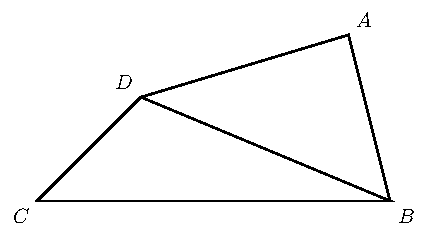
\includegraphics[height=4cm,page=1]{aops-amc10-figure-1}
\end{center}
\bigskip

\begin{answer}
%Project $D$ onto $CB$ to point $D^{\prime}$. 
Project $A$ onto $BD$ to point $A^{\prime}$. 
Let $x$ denote the unknown $BD$, $y$ the segment $BA^{\prime}$, and let $h$ denote the height $AA^{\prime}$. 
%Likewise, let $z$ denote the segment $CD^{\prime}$, and let $k$ denote the height $DD^{\prime}$. 
\bigskip
\begin{center}
  \includegraphics[height=8cm,page=2]{aops-amc10-figure-1}
\end{center}
\bigskip
Applying the Pythagoras theorem to triangles 
% $DD^{\prime}C$, $DD^{\prime}B$, 
$AA^{\prime}B$, and $AA^{\prime}D$ yields:
\begin{align*}
        h^2 + y^2 & = 5^2 
 \\ h^2 + (x-y)^2 & = 9^2 
%     \\ k^2 + z^2 & = 5^2 
%\\ k^2 + (17-z)^2 & = x^2 
\end{align*}
The first equation may be subtracted from the first to eliminate $h$ and get an expression in $x$ and $y$. 
%And likewise with the other two equations.
\begin{align*}
    (x-y)^2 - y^2 & = 9^2 - 5^2
%\\ (17-z)^2 - z^2 & = x^2 - 5^2 
\\      x^2 - 2yx & = 56 
%\\ x^2 + 34z & = 314
\end{align*}
Since we know that $x$ is an integer, we can guess its value as follows. Factor $x$ and write $56$ as the product of its prime factors. 
\begin{align*}
x(x - 2y) = 2^3 \times 7
\end{align*}
We guess $x=2^3$ and $x-2y=7$.
\end{answer}
%%%%%%%%%%%%%%%%%%%%%%%%%%%%%%%%%%%%%%%%%%%%%%%%%%%%%%%%%%%%%%%%%%%%%%%%

\iftoggle{showAnswers}{\newpage}
\end{comment}


\end{document}